% Copyright (c)  2005-2010 EDF-EADS-PHIMECA.
% Permission is granted to copy, distribute and/or modify this document
% under the terms of the GNU Free Documentation License, Version 1.2
% or any later version published by the Free Software Foundation;
% with no Invariant Sections, no Front-Cover Texts, and no Back-Cover
% Texts.  A copy of the license is included in the section entitled "GNU
% Free Documentation License".
\renewcommand{\filename}{docUC_InputNoData_CopulaEstimation.tex}
\renewcommand{\filetitle}{UC : Estimating a Copula from a sample}

% \HeaderNNIILevel
% \HeaderIILevel
\HeaderIIILevel


\label{copula_estimation}


\index{Copula!Estimation from a sample}
\index{Graph Manipulation!Bounding box}
\index{Graph Manipulation!ViewImage}
\index{Graph Manipulation!Show}
\index{Fitting Test!QQ-plot}
\index{Fitting Distribution!Parametric method}



The objective of this Use Case is to :
\begin{itemize}
\item fit a copula to a sample : this estimation may be parametric (when using a specific model of copula) or not (when using the Sklar Copula),
\item validate these estimations with a visual test by superposing the clouds composed by the ranked points of the sample and the iso-curves of the estimated copula.
\end{itemize}


Details on the Maximum Likelihood  Principle may be found in the Reference Guide (\href{OpenTURNS_ReferenceGuide.pdf}{see files Reference Guide - Step B -- Maximum Likelihood  Principle}).\\

Details on the Parametric Estimators used to evaluate the parameters of the copula may be found in the Reference Guide (\href{OpenTURNS_ReferenceGuide.pdf}{see files Reference Guide - Step B --  Parametric Estimation}).\\

Details on each object may be found in the User Manual  (\href{OpenTURNS_UserManual_TUI.pdf}{see User Manual - Statistics on sample /  Distribution factory}).\\


In the example, we suppose we have a sample of dimension 2 and that we have already performed the analysis marginal by marginal in order to estimate the marginal distributions of the sample. The objective, now, is to estimate the dependence structure of the points. The analysis  have the following steps :
\begin{enumerate}
\item transform the sample into the ranked sample, using the marginal distributions,
\item estimate the dependence structure with a parametric or not parametric method,
\item validate the estimation by superposing on the ranked sample cloud the iso-curves of the estimated copula.
\end{enumerate}


Let's note that there exists different methodologies to estimate a $nD$ distribution from a sample.


\requirements{
  \begin{description}
  \item[$\bullet$] a 2D numerical sample (data) : {\itshape sample}
  \item[type:]  NumericalSample
  \end{description}
}
{
  \begin{description}
  \item[$\bullet$] a Copula : {\itshape estimatedCopula}
  \item[type:] CopulaImplementation : Frank, Clayton, Gumbel, Independent, Normal, Sklar.
  \end{description}
}

\textspace\\
Python script for this UseCase :

\begin{lstlisting}
  # Creation of the operator which transforms the marginals into the uniform ones
  # We suppose here that the marginal distributions are both Normal(0,1)
  ranksTransf = MarginalTransformationEvaluation(DistributionCollection([Normal(), Normal()]), MarginalTransformationEvaluation.FROM)

  # Transformation of the initial sample into the ranked sample
  transformedSample = NumericalSample(initSample.getSize(), initSample.getDimension())
  for i in range(initSample.getSize()) :
  transformedSample[i] = ranksTransf(initSample[i])

  # Cloud of the ranked points
  rankedCloud = Cloud(transformedSample, 'blue', 'plus', 'ranks sample')
  myGraph = Graph('Parametric estimation of the copula', 'X', 'Y', True, 'topleft')
  myGraph.addDrawable(rankedCloud)

  # Estimation of a copula on the ranked points cloud
  # For example, a parametric estimation : the Clayton Copula
  estimatedCopula = ClaytonCopulaFactory().build(transformedSample)
  print estimatedCopula

  # Superposition of the iso-curves of the copula estimated on the points cloud
  minPoint = NumericalPoint([0.0, 0.0])
  maxPoint = NumericalPoint([1.0, 1.0])
  pointNumber = NumericalPoint([201, 201])
  graphEstimatedCopula = estimatedCopula.drawPDF(minPoint, maxPoint, pointNumber)
  contour_estimatedCopula = graphEstimatedCopula.getDrawable(0)
  contour_estimatedCopula.setDrawLabels(False)

  # Change the levels of the iso-curves
  # Levels of the iso curves
  nlev = 31
  levels = NumericalPoint(nlev)
  for i in range(nlev):
  levels[i] = 0.25 * nlev / (1.0 + i)

  contour_estimatedCopula.setLevels(levels)

  # Change the legend of the curves
  contour_estimatedCopula.setLegendName('Clayton copula iso-PDF')
  graphEstimatedCopula.setDrawable(contour_estimatedCopula, 0)

  # Change the color of the iso-curves
  graphEstimatedCopula_draw = graphEstimatedCopula.getDrawable(0)
  graphEstimatedCopula_draw.setColor('red')

  # Add the iso-curves graph into the cloud one
  myGraph.addDrawable(graphEstimatedCopula_draw)
  myGraph.setLegendPosition('bottomright')

  # Visualize the graph
  Show(myGraph)

  # Print the graph in file.PNG
  myGraph.draw('copula_estimation', 640, 480, GraphImplementation.PNG)
\end{lstlisting}
\textspace\\


Figure \ref{InitCloud} gives the cloud of the sample and Figure \ref{RankCloud} gives the cloud of the ranks. Figure \ref{Superposition} gives the superposition of the ranks cloud and the iso-curves of the estimated copula.



\begin{figure}[H]
  \begin{minipage}{10cm}
    \begin{center}
      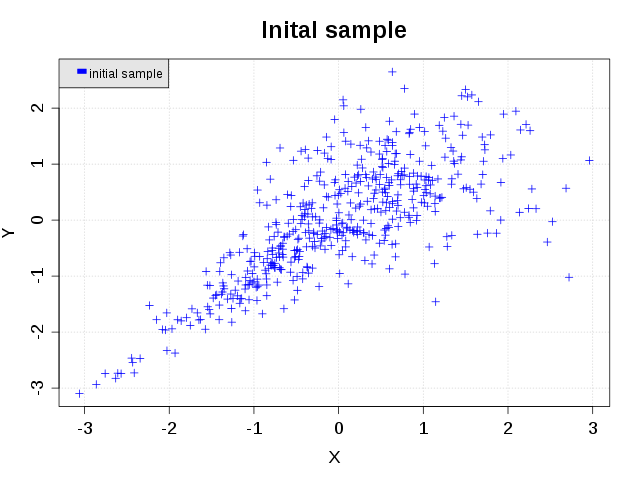
\includegraphics[width=10cm]{initSample.png}
    \end{center}
    \caption{Initial sample.}
    \label{InitCloud}
  \end{minipage}
  \hfill
  \begin{minipage}{10cm}
    \begin{center}
      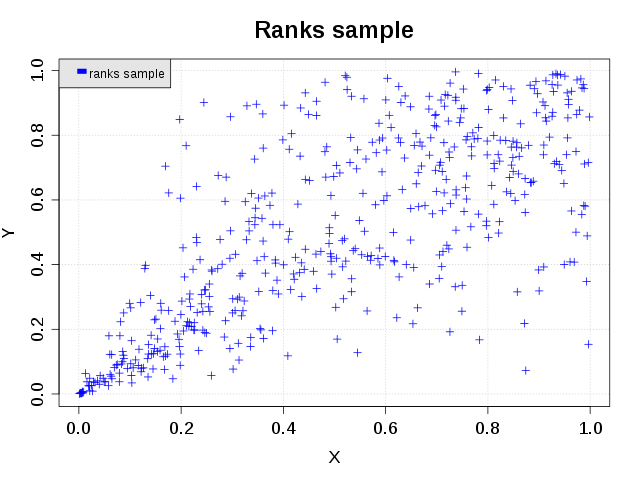
\includegraphics[width=10cm]{ranksSample.png}
    \end{center}
    \caption{Clouds of the ranked points.}
    \label{RankCloud}
  \end{minipage}
\end{figure}


\begin{figure}[H]
  \begin{center}
    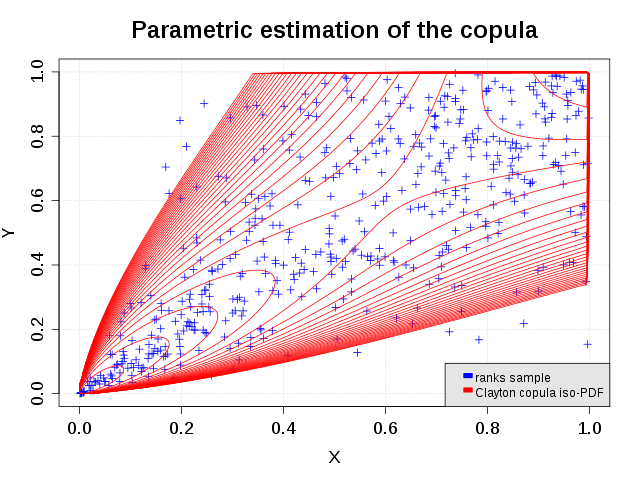
\includegraphics[width=10cm]{copula_estimation.png}
  \end{center}
  \caption{Ranked points and iso-curves of the PDF of the estimated copula.}
  \label{Superposition}
\end{figure}
